\chapter{Modelo de Negócios}

O modelo de negócios de uma empresa basicamente define onde uma empresa executa e vende seus produtos e (ou) serviços. Além disso, deve mostrar o valor que o produto (ou serviço) oferece para os seus clientes, definindo de que forma a empresa lucrará ao entregar esse valor para seus consumidores. Em outra palavras, a empresa irá definir o que fazer, porque fazer e como fazer, traçando uma linha de objetivos e caminhos a serem seguidos pela empresa. O modelo é útil tanto para empresas grandes que precisam reduzir custos, redefinir estratégias, entre outros, quanto para empresas iniciantes, que precisam definir suas diretrizes e, muitas vezes, de um grande documento que apresente os recursos necessários para dar início à empresa~\cite{modelo_de_negocios}.

Existem alguns métodos para se definir um modelo de negócios, sendo que em sua maioria, são técnicas complementares. A mais conservadora é a criação de um plano de negócios, técnica muito difundida e utilizada. Porém, nos dias de hoje, uma outra técnica vem ganhando muito espaço, o BMC (\textit{Business Model Canvas}).
\abbrev{BMC}{Business Model Canvas}
A seguir serão apresentadas vantagens e desvantagens de cada um destes métodos, visando permitir uma melhor análise comparativa entre eles~\cite{comparabmcplanoum}~\cite{comparabmcplanodois}.

\section{Plano de Negócios}

O plano de negócios tem como objetivo especificar em detalhes o negócio que está sendo analisado. Por esse motivo, ao final do processo é gerado um documento muito extenso e explicativo relativo a todas as áreas da empresa. Além de uma explicação detalhada da empresa, seus objetivos e propostas de valor, sua produção pressupõe a criação de um plano financeiro, plano de marketing, plano de recursos humanos e um cronograma completo.

\subsection{Vantagens}

\begin{itemize}
\item Facilidade na aquisição de investimentos para o negócio, já que, além de mais detalhes, apresenta um plano financeiro, explicitando gastos e previsões sobre o tempo de retorno.
\item Ajuda a prever todas as áreas da empresa, tendo uma visão macro do negócio e aumentando o entendimento dos sócios em cada área.
\end{itemize}

\subsection{Desvantagens}

\begin{itemize}
\item É um processo muito demorado e requer muita pesquisa. Pode demorar semanas ou até meses para ser criado.
\item Muitas vezes, os sócios ainda não têm conhecimento sobre algumas hipóteses, podendo levar à criação de um plano inconsistente e irreal.
\item Diversas variáveis mudam com o tempo e são imprevisíveis, de forma que o plano pode se desatualizar rapidamente.
\item Os sócios, em geral, acabam utilizando informações incorretas ou não embasadas em diversos pontos do plano, gerando um documento muitas vezes inconsistente.
\item Se ocorre uma mudança na empresa, é necessário mudar todo o plano, tendo um custo de atualização altíssimo.
\end{itemize}

\section{BMC}

Inicialmente proposto por Alexander Osterwalder, o BMC visa produzir o modelo de negócios rapidamente e de forma dinâmica. O documento final é de apenas uma folha pré-formatada com nove blocos que definem o modelo de negócios. São eles: principais atividades, principais recursos, rede de parceiros, proposição de valor, segmentos de clientes, canais, relacionamento com o cliente, estrutura de custos e fluxos de receita. A ideia sugere a utilização de \textit{post-its} para que definições possam ser alteradas com facilidade.~\cite{tutorialbmc}

\subsection{Vantagens}

\begin{itemize}
\item Velocidade de produção, já que contém apenas uma folha com um padrão claro de preenchimento.
\item Modelo preparado para mudanças ao longo do processo, considerando que um empreendedor nem sempre já tem de início o conhecimento necessário na área onde estará atuando.
\item Cria um documento enxuto, isto é, focado apenas no que é mais importante, evitando perda de tempo com detalhes que têm grandes chances de serem alterados.
\item Por estar sempre sendo revisado, propicia a inovação e melhoria das ideias sobre a empresa.
\end{itemize}

\subsection{Desvantagens}

\begin{itemize}
\item Por ser um documento de criação simples e rápida, muito vezes acaba sendo superficial.
\item Pode conter dados inconsistentes, visto que os criadores nem sempre estudam e pesquisam a respeito da área de atuação.
\item Ainda não é visto por investidores como um substituto do plano de negócios, tornando necessário o desenvolvimento do plano mais completo na hora de angariar recursos.
\end{itemize}

\section{Blocos do BMC}

\subsection{Principais Atividades}

Este bloco visa definir todas as atividades que são necessárias para executar o modelo de negócios da empresa. Basicamente, estas atividades fazem com que todas as informações descritas nos outros blocos sejam alcançadas.

\subsection{Principais Recursos}

Esta área do documento tem como objetivo explicitar todos os recursos necessários para entregar o devido valor para seus clientes e ter uma renda em cima disso. Os itens dessa seção devem incluir recursos tangíveis e até mesmo os intangíveis. Em geral existem quatro categorias de recursos:

\begin{itemize}
\item Recursos Físicos

Envolvem máquinas, escritórios, instalações, entre outros.

\item Recursos Intelectuais

Neste são consideradas marcas, patentes ou informações (em um BD, por exemplo). Apesar da dificuldade de se gerar recursos intelectuais, uma vez gerados, são muito valiosos.

\item Recursos Humanos

Como o próprio nome já diz, visa definir os empregados necessários para o funcionamento da empresa.

\item Recursos Financeiros

Definem valores como investimentos ou linhas de crédito, necessários para tirar a empresa do papel e colocá-la para funcionar.
\end{itemize} 

\subsection{Rede de Parceiros}

A rede de parceiros tem como objetivo definir quem são fornecedores e parceiros que fazem o modelo funcionar melhor. Isso pode envolver possíveis parcerias com não-concorrentes, concorrentes, fornecedores e compradores. Como motivação para as parcerias, pode-se considerar:

\begin{itemize}
\item Otmização e escala devido à melhor alocação de recursos e redução de custos.
\item Para tentar minimizar o risco e as incertezas do projeto, é comum a parceria entre empresas concorrentes.
\item Ao invés de desenvolver novas atividades na empresa, muitas vezes é melhor focar no que se sabe fazer, e criar uma parceria com quem o complemente. Então, ao criar parcerias, estendem-se a capacidade e as atividades da empresa.
\end{itemize}

\subsection{Proposição de Valor}

Esta seção é alma do documento. Nela está descrita a proposta de valor entregue ao cliente através do produto, ou seja, é o valor observado pelo cliente no produto ou serviço oferecido. Consequentemente, é determinante na aquisição de novos clientes. Diversos elementos podem contribuir à proposta de valor, como: inovação, design, preço, usabilidade, entre outros.

\subsection{Segmentos de Clientes}

Essa área visa definir quem são os consumidores e clientes da empresa. Numa situação de um crescimento muito grande da base de clientes, se torna interessante dividí-los em segmentos de forma a atendê-los melhor. Os segmentos podem ser de massa (não há distinção de clientes), de nicho (focado em uma área de atuação), diversificados (que atendem diversas áreas) ou até mesmo mercados multilaterais (que trabalham com mais de um segmentos para funcionar).

\subsection{Canais}

Como o próprio nome já diz, visa definir os canais de comunicação, distribuição e venda do produto ou serviço. Eles são muito importantes para saber com clareza por onde o consumidor irá conhecer o produto, onde irá adquirí-lo e por onde poderá dar um feedback. É importante avaliar por onde aumentar a base de clientes, como de fato passar a proposta de valor ao cliente, como entregar esse valor e como dar suporte ao consumidor. Dessa forma, todo o canal de comunicação estará definido.

\subsection{Relacionamento com o Cliente}

Este bloco define que tipo de relacionamento com o cliente ocorrerá. Existem diversas possibilidades, como uma assistência pessoal, comunidades (consumidores se ajudam) ou até mesmo por meio de auto ajuda, onde a empresa oferece meios ao consumidor para descobrir sozinho o que precisa.

\subsection{Estrutura de Custos}

Esta parte do BMC tenta definir quais são os gastos necessários para o bom funcionamento da empresa. Além disso, tenta encontrar recursos e atividades que são muito caros. Se o resto do documento já estiver preenchido, se torna mais fácil definir a estrutura de custos. Basicamente, existe em empresas focadas em reduzir custos e empresas focadas em agregar valor ao seu produto ou serviço. As duas formas visam aumentar o lucro, porém de maneira oposta.

É importante também dar o devido valor ao tipo de custo, isto é, se é um custo fixo, onde os custos se mantém ao longo do tempo, ou variável, que variam de acordo com o volume de produto ou serviço.

\subsection{Fluxos de Receita}

Fluxos de receita definem a renda gerada por cada segmento de clientes, definindo quanto cada um deles está disposto a pagar pela proposta de valor. As fontes de receita podem ser geradas de diversas formas, desde uma venda específica, venda de assinaturas, venda de anúncios ou até mesmo licenciando o produto ou serviço da empresa.

\section{Modelo de Negócios do EVNTs}

Neste capítulo, será apresentado o modelo de negócios do projeto. Primeiramente, analisando as vantagens e desvantagens, foi escolhido aplicar o BMC, já que o trabalho é focado em desenvolvimento ágil. Além disso, o BMC é interessante por facilitar modificações futuras, que certamente ocorrerão. O BMC produzido pode ser visualizado na ~\ref{fig:bmc}.

\begin{figure}[H]
\centering
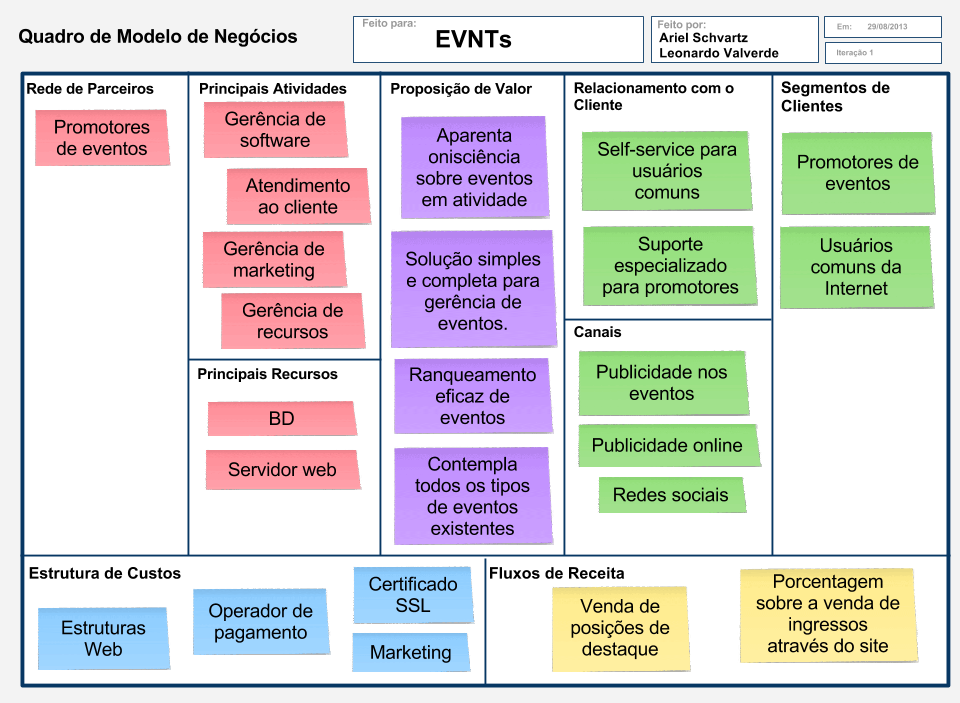
\includegraphics[width=1\textwidth]{figs/bmc}
\caption[\textit{BMC do projeto}]
{BMC do projeto}
\label{fig:bmc}
\end{figure}

Como o BMC é uma representação muito sucinta do negócio, será realizado a seguir um detalhamento de cada tópico incluído no mesmo.

\begin{itemize}

\item Proposições de Valor

\begin{itemize}

\item Aparenta onisciência sobre os eventos em atividade

Obviamente, é essencial para o sucesso da aplicação que nela estejam cadastrados muitos eventos. De forma ideal, pode-se imaginar o caso extremo, onde todos os eventos existentes estão mapeados na aplicação.

\item Ranqueamento eficaz de eventos

De nada adianta mapear boa parte dos eventos existentes sem um ranqueamento eficiente. É humanamente impossível detectar eventos interessantes dentre uma lista não ordenada contendo todos os eventos em atividade. A ferramenta de ranqueamento é vital para o sucesso da aplicação.

\item Contempla todos os tipos de eventos existentes

Como citado anteriormente, uma das grandes deficiências dos sistemas vigentes que auxiliam na gerência de eventos é a sua pouca versatilidade. A aplicação deve dar suporte aos diferentes tipos de eventos existentes, de forma a permitir manutebilidade ao seu gerenciamento.

\item Solução simples e completa para a gerência de eventos

Um dos principais focos é oferecer todas as ferramentas demandadas pelo usuário, no que diz respeito à gerência de eventos. A ideia é que os usuários não precisem utilizar nenhuma outra plataforma para realizar tal tarefa.

\end{itemize}

\item Principais Recursos

\begin{itemize}

\item Banco de Dados

O Banco de Dados é um recurso essencial para o funcionamento do sistema. Além disso, é responsável pelo armazenamento de informações, sendo um recurso intelectual de extrema importância.
\item Servidor Web

Além do BD, o servidor é o outro pilar essencial para que um sistema web funcione plenamente. Dessa forma, se torna outro recurso essencial para o modelo de negócios. Sua escolha afeta a manutenção, custo e escalabilidade do projeto.
\end{itemize}

\item{Segmentos de Clientes}

\begin{itemize}
\item Usuários Comuns da Internet

O aplicativo foca em prover funcionalidades úteis a qualquer pessoa. Ou seja, em um primeiro momento, qualquer um que esteja conectado à Internet poderá se interessar por usar o EVNTs, caracterizando-se assim, um segmento de massa.

\item Promotores de Eventos

Os promotores de eventos são usuários organizadores de grandes eventos públicos e pagos, sendo assim extremamente valiosos para o projeto. Dessa forma, são os usuários que, provavelmente, criarão os eventos com a maior quantidade de pessoas confirmadas dentro do sistema. Assim, além de serem grandes geradores de renda (ver a parte de fluxos de receita) serão atrativos para novos usuários.
\end{itemize}

\item{Rede de Parceiros}

\begin{itemize}
\item Promotores de Eventos

Além de usuários do sistema, organizando eventos, os promotores podem ser considerados também parceiros. São pessoas de suma importância para a criação de uma grande base de eventos, pois através de uma relação de benefício mútuo, os promotores encontram no sistema um local para divulgação e venda de ingressos, enquanto atraem novos clientes a este.
\end{itemize}

\item{Canais}

\begin{itemize}
\item Publicidade nos Eventos

Este canal visa fazer um contato \textit{offline} com os clientes. A ideia é que em grandes festas, shows e outros eventos públicos, sejam colocadas propagandas (como cartazes e banners) de forma a mostrar aos usuários, por exemplo, que poderiam ter adquirido ingressos por meio da aplicação.

\item Publicidade \textit{Online}

Uma das formas mais utilizadas para divulgação de aplicativos web é a realização desta por meio de propagandas em sites. É um método extremamente eficiente, pois basta um clique para que o usuário acesse o sistema. Existem empresas muito populares que proveem este serviço, proporcionando ao contratante um grau de visibilidade proporcional ao pagamento realizado.

\item Redes Sociais

As redes sociais vêm cada vez mais se tornando o principal meio de divulgação para micro e pequenas empresas, já que são baratas (ou até mesmo gratuitas) e, com dedicação, é possível uma boa alcançabilidade. 

\end{itemize}

\item{Relacionamento com o Cliente}

\begin{itemize}
\item Auto ajuda para usuários comuns

Em geral, como teremos uma gama muito grande de usuários, torna-se muito custosa a criação de um sistema de suporte pessoal. Porém, por dispor de diversas funcionalidades inéditas pelos usuários, é importante que se estabeleça um relacionamento através de um sistema auto ajuda, como um FAQ (\textit{Frequently Asked Questions})
~\abbrev{FAQ}{\textit{Frequently Asked Questions}}
para auxiliá-los.

\item Suporte Especializado para Promotores

Por terem uma importância muito grande para o sistema, é essencial oferecer atendimento especial aos promotores, além de suporte personalizado, de forma a deixá-los a vontade com o sistema e sem dúvidas sobre o funcionamento do mesmo.

\end{itemize}

\item{Principais atividades}

\begin{itemize}
\item Gerência de \textit{Software}

Se faz necessária uma equipe de desenvolvimento e manutenção do \textit{software}, para garantir o seu bom funcionamento, além de proporcionar melhorias ao mesmo.

\item Atendimento ao Cliente

É necessária uma equipe voltada para o relacionamento com os clientes, citado anteriormente. Isso inclui esforços tanto para a manutenção do sistema de auto ajuda como para o contato direto com os promotores.

\item Gerência de Marketing

Equipe especializada em estudar locais (\textit{online} e \textit{offline}) para divulgação do sistema, além de criar campanhas nos mesmos, inclusive em redes sociais.

\item Gerência de Recursos

É essencial que o caixa da empresa seja gerenciado de forma inteligente. Para isso é necessário que haja uma equipe voltada para a gerência de recursos do projeto, distribuindo-os ao longo dos demais setores da empresa.

\end{itemize}

\item{Fluxos de Receita}

\begin{itemize}

\item Porcentagem sobre a Venda de Ingressos

A principal fonte de receita da empresa, se baseia na venda de ingressos. Basicamente, seria cobrado um percentual do valor do ingresso pelos serviços sendo prestados. O organizador, pode optar por incluir esse valor ao preço do ingresso ou deixar que o usuário pague por ele.

\item Venda de Posições de Destaque

Outra forma de gerar receita, seria através da venda de posições de destaque para eventos. Com isso, haveria uma área no site de ``Eventos em Destaque'' com os eventos que pagaram para ter aquela posição especial.

\end{itemize}

\item{Estrutura de Custos}

\begin{itemize}

\item Estruturas Web

Os gastos em estruturas web basicamente são representados com: servidor, banco de dados e domínio.

\item Operador de Pagamento

O operador de pagamento, em um primeiro momento, será o PayPal por seu selo de segurança e praticidade de implementação. Porém, é um custo muito alto para a empresa, já que o valor cobrado é de 5,4\% a 6,4\% + R\$0,60 por transação. É importante ter em mente que se faz necessária a pesquisa por outras soluções de pagamento, para não inviabilizar o projeto.

\item Certificado SSL

Como explicado na parte de segurança do Rails, é importante o uso de conexões SSL, para que informações se tornem criptografadas e, consequentemente, seguras. Para que o usuário saiba que um site é criptografado, existem empresas que vendem certificados SSL, atestando a segurança do mesmo.

\item Marketing

Marketing é um dos principais gastos de qualquer empresa que quer crescer rapidamente. Além dos gastos com uma equipe, existem diversos outros relacionados aos meios de divulgação e a produção de campanhas.

\end{itemize}

\end{itemize}
